% ============================================================
% Blockchain-Based Shipment Tracking System — Technical Report
% CSE 540 – Engineering Blockchain Applications
% Arizona State University | Spring B 2026 | Group 1
%
% IEEE 2-column format, 4–8 pages
% Compile with: pdflatex REPORT.tex (run twice for references)
% ============================================================

\documentclass[conference]{IEEEtran}

% ── Packages ──
\usepackage[utf8]{inputenc}
\usepackage[T1]{fontenc}
\usepackage{lmodern}
\usepackage{graphicx}
\usepackage{xcolor}
\usepackage{tikz}
\usetikzlibrary{shapes.geometric, arrows.meta, positioning, calc, fit, matrix, backgrounds, shadows, decorations.pathreplacing}
\usepackage{pgfplots}
\pgfplotsset{compat=1.18}
\usepackage{enumitem}
\usepackage{booktabs}
\usepackage{tabularx}
\usepackage{hyperref}
\usepackage{listings}
\usepackage{amssymb}
\usepackage{pifont}
\usepackage{float}
\usepackage{caption}
\usepackage{amsmath}
\usepackage{balance}
\usepackage{url}
\usepackage{multirow}

% ── Colors ──
\definecolor{fabricblue}{RGB}{41,98,255}
\definecolor{darkgreen}{RGB}{0,128,0}
\definecolor{codebg}{RGB}{245,245,245}
\definecolor{asumaroon}{RGB}{140,28,19}
\definecolor{asugold}{RGB}{255,198,39}
\definecolor{nodeblue}{RGB}{173,216,230}
\definecolor{nodeorange}{RGB}{255,220,177}
\definecolor{nodegreen}{RGB}{198,239,206}
\definecolor{nodepurple}{RGB}{220,198,239}
\definecolor{nodegray}{RGB}{230,230,230}
\definecolor{nodered}{RGB}{255,199,206}

% ── Hyperlinks ──
\hypersetup{
    colorlinks=true,
    linkcolor=black,
    citecolor=black,
    urlcolor=fabricblue,
}

% ── Code Listings ──
\lstset{
    basicstyle=\ttfamily\scriptsize,
    backgroundcolor=\color{codebg},
    frame=single,
    rulecolor=\color{gray!40},
    breaklines=true,
    showstringspaces=false,
}

\newcommand{\cmark}{\ding{51}}
\newcommand{\xmark}{\ding{55}}

% ════════════════════════════════════════════════════════════════
\begin{document}

% ── Title ──
\title{Blockchain-Based Shipment Tracking System:\\A Hyperledger Fabric Approach to Supply Chain Provenance}

\author{
    \IEEEauthorblockN{Dominick Agnello, Ritish Abrol, Vatsal Patel, Shashikant Nanda, Anushree Bhure}
    \IEEEauthorblockA{
        CSE 540 -- Engineering Blockchain Applications\\
        Ira A. Fulton Schools of Engineering, Arizona State University\\
        Spring B 2026 -- Group 1\\
        Repository: \url{https://github.com/Blugil/group1-cse540-blockchain}
    }
}

\maketitle

% ════════════════════════════════════════════════════════════════
%  ABSTRACT
% ════════════════════════════════════════════════════════════════
\begin{abstract}
Modern supply chains suffer from fragmented record-keeping, lack of transparency, and trust deficits among participating organizations. Each entity---manufacturer, transporter, warehouse, retailer---maintains its own isolated database, creating opportunities for fraud, data tampering, and unresolvable disputes. This paper presents a blockchain-based shipment tracking system built on Hyperledger Fabric 2.5 that provides an immutable, shared ledger for recording every custody transfer, status update, and participant authorization across the supply chain. Our smart contract, implemented in Go (647 lines), enforces role-based access control (RBAC) via MSP identities, maintains data integrity through SHA-256 off-chain hashing, and stores a complete event history using composite keys. The system is validated through 15 unit tests using Fabric's MockStub framework with mock X.509 identities. We provide a quantitative analysis comparing our blockchain approach against traditional centralized database solutions, evaluate scalability and transaction throughput characteristics, and discuss privacy and regulatory considerations. Results demonstrate that the system successfully enforces tamper-proof provenance tracking with sub-second transaction latency while eliminating single points of trust failure.
\end{abstract}

\begin{IEEEkeywords}
Hyperledger Fabric, supply chain management, blockchain, smart contract, provenance, shipment tracking, RBAC, SHA-256
\end{IEEEkeywords}

% ════════════════════════════════════════════════════════════════
%  I. INTRODUCTION
% ════════════════════════════════════════════════════════════════
\section{Introduction}

Global supply chains involve multiple independent organizations---manufacturers, transporters, warehouses, retailers, and end recipients---each maintaining its own record-keeping system. This fragmentation creates a fundamental trust problem: when a shipment is lost, damaged, or disputed, no single authoritative record exists to resolve the conflict. The World Economic Forum estimates that eliminating supply chain barriers could increase global trade by nearly 15\% \cite{shakhbulatov2020}.

Blockchain technology offers a compelling solution by providing a shared, append-only ledger that no single party controls. However, public blockchains like Ethereum are unsuitable for enterprise supply chains due to their lack of privacy controls, high gas fees, and limited throughput ($\sim$30 TPS) \cite{oguz2024}. Hyperledger Fabric, a permissioned blockchain framework maintained by the Linux Foundation, addresses these limitations through its channel-based privacy model, identity management via Membership Service Providers (MSPs), and modular consensus architecture capable of thousands of transactions per second \cite{gonczol2020}.

Fig.~\ref{fig:highlevel} presents the high-level concept of our solution, replacing the traditional fragmented model with a unified blockchain backbone.

\begin{figure}[htbp]
\centering
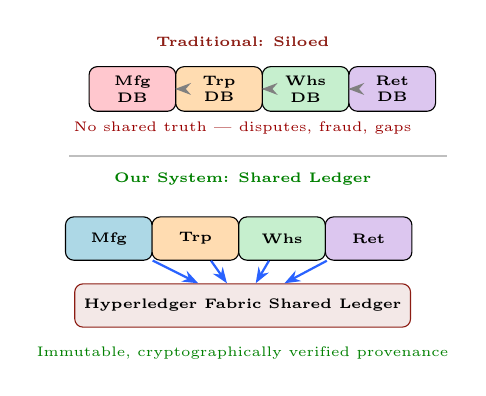
\begin{tikzpicture}[
  actor/.style={rectangle, draw=black, rounded corners=3pt, fill=#1, minimum width=1.1cm, minimum height=0.55cm, font=\tiny\bfseries, align=center},
  arr/.style={-{Stealth[length=2mm]}, thick},
  dbarr/.style={-{Stealth[length=2mm]}, thick, dashed, gray},
  lbl/.style={font=\tiny, align=center},
]
  % Traditional (top)
  \node[lbl, text=asumaroon] at (0,2.2) {\textbf{Traditional: Siloed}};
  \node[actor=nodered] (mfg)  at (-1.4,1.6) {Mfg\\DB};
  \node[actor=nodeorange] (trp) at (-0.3,1.6) {Trp\\DB};
  \node[actor=nodegreen] (whs) at (0.8,1.6)  {Whs\\DB};
  \node[actor=nodepurple] (ret) at (1.9,1.6) {Ret\\DB};
  \draw[dbarr] (mfg) -- (trp);
  \draw[dbarr] (trp) -- (whs);
  \draw[dbarr] (whs) -- (ret);
  \node[lbl, text=red!60!black] at (0,1.1) {No shared truth — disputes, fraud, gaps};

  % Divider
  \draw[thick, gray!50] (-2.2,0.75) -- (2.6,0.75);

  % Blockchain (bottom)
  \node[lbl, text=darkgreen] at (0,0.45) {\textbf{Our System: Shared Ledger}};
  \node[actor=nodeblue] (m2)  at (-1.7,-0.3) {Mfg};
  \node[actor=nodeorange] (t2) at (-0.6,-0.3){Trp};
  \node[actor=nodegreen] (w2) at (0.5,-0.3) {Whs};
  \node[actor=nodepurple] (r2) at (1.6,-0.3){Ret};
  \node[rectangle, draw=asumaroon, fill=asumaroon!10, rounded corners=3pt,
        minimum width=3.5cm, minimum height=0.55cm, font=\tiny\bfseries]
        (bc) at (0,-1.15) {Hyperledger Fabric Shared Ledger};
  \draw[arr, fabricblue] (m2) -- (bc);
  \draw[arr, fabricblue] (t2) -- (bc);
  \draw[arr, fabricblue] (w2) -- (bc);
  \draw[arr, fabricblue] (r2) -- (bc);
  \node[lbl, text=darkgreen] at (0,-1.75) {Immutable, cryptographically verified provenance};
\end{tikzpicture}
\caption{High-level concept: siloed databases vs.\ shared blockchain ledger.}
\label{fig:highlevel}
\end{figure}

Our contributions include:
\begin{enumerate}[nosep, leftmargin=*]
    \item A fully implemented Go chaincode with 10 functions enforcing RBAC, custody transfer logic, and SHA-256 data integrity verification.
    \item A three-layer system architecture comprising a Node.js REST API, a Hyperledger Fabric network with Raft consensus, and a Certificate Authority-based identity layer.
    \item A comprehensive test suite of 15 unit tests validating all business logic including edge cases and a full lifecycle scenario.
    \item A quantitative comparison between our blockchain solution and a traditional centralized database approach.
\end{enumerate}

% ════════════════════════════════════════════════════════════════
%  II. PRIOR WORK
% ════════════════════════════════════════════════════════════════
\section{Prior Work}

Blockchain-based supply chain management has received significant research attention. Shakhbulatov et al.\ \cite{shakhbulatov2020} survey how blockchain enhances supply chain management through immutability, transparency, and decentralized trust, noting permissioned platforms like Hyperledger Fabric are preferred for enterprise deployments.

Oguz et al.\ \cite{oguz2024} systematically review 148 studies, finding Hyperledger Fabric is used in 42\% of permissioned supply chain implementations, with scalability, interoperability, and regulatory compliance as primary challenges.

Gonczol et al.\ \cite{gonczol2020} recommend hybrid on-chain/off-chain architectures---a pattern our system adopts via SHA-256 hash-based verification. Wang et al.\ \cite{wang2019} propose a Fabric-based food traceability system focused on IoT integration; unlike their approach, our system emphasizes dynamic participant authorization and post-delivery immutability.

Our work adds explicit chaincode-level RBAC, composite-key event storage, and a comprehensive test suite that validates all rules without requiring a live network.

% ════════════════════════════════════════════════════════════════
%  III. TECHNICAL ARCHITECTURE
% ════════════════════════════════════════════════════════════════
\section{Technical Architecture}

\subsection{Three-Layer System Architecture}

Fig.~\ref{fig:architecture} shows the three layers of our system.

\begin{figure}[htbp]
\centering
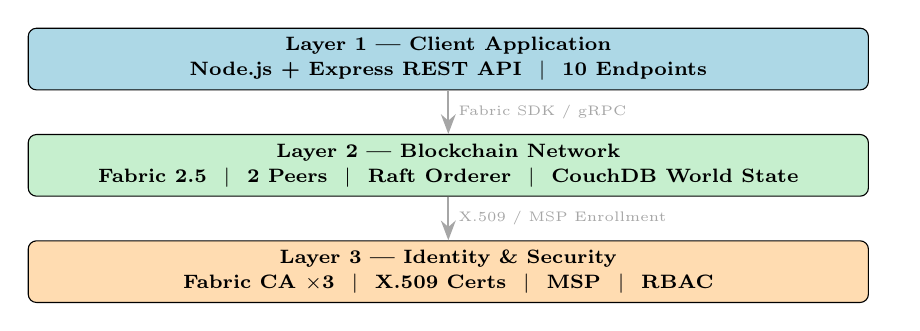
\begin{tikzpicture}[
  box/.style={rectangle, draw=black, rounded corners=3pt, fill=#1,
              minimum width=\columnwidth*0.88, minimum height=0.72cm,
              font=\scriptsize\bfseries, align=center},
  sub/.style={rectangle, draw=gray!60, fill=white, rounded corners=2pt,
              font=\tiny, align=center, minimum width=1.5cm, minimum height=0.4cm},
  arr/.style={-{Stealth[length=2.5mm]}, thick, gray!70},
]
  \node[box=nodeblue] (l1) at (0,0)
    {Layer 1 — Client Application\\[1pt]
     \scriptsize Node.js + Express REST API \ $|$ \ 10 Endpoints};

  \node[box=nodegreen] (l2) at (0,-1.35)
    {Layer 2 — Blockchain Network\\[1pt]
     \scriptsize Fabric 2.5 \ $|$ \ 2 Peers \ $|$ \ Raft Orderer \ $|$ \ CouchDB World State};

  \node[box=nodeorange] (l3) at (0,-2.7)
    {Layer 3 — Identity \& Security\\[1pt]
     \scriptsize Fabric CA $\times$3 \ $|$ \ X.509 Certs \ $|$ \ MSP \ $|$ \ RBAC};

  \draw[arr] (l1) -- node[right, font=\tiny] {Fabric SDK / gRPC} (l2);
  \draw[arr] (l2) -- node[right, font=\tiny] {X.509 / MSP Enrollment} (l3);

  % Side labels
  \node[font=\tiny, text=gray, right=0.05cm of l1] {};
\end{tikzpicture}
\caption{Three-layer system architecture.}
\label{fig:architecture}
\end{figure}

\subsection{Fabric Network Topology}

Fig.~\ref{fig:topology} details the internal network components and their connections.

\begin{figure}[htbp]
\centering
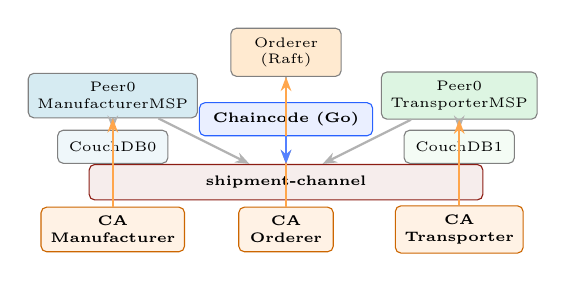
\begin{tikzpicture}[
  org/.style={rectangle, draw=#1!80!black, fill=#1!15, rounded corners=4pt,
              inner sep=4pt, font=\tiny\bfseries},
  node/.style={rectangle, draw=gray, fill=white, rounded corners=2pt,
               font=\tiny, align=center, minimum width=1.4cm, minimum height=0.42cm},
  ca/.style={rectangle, draw=orange!80!black, fill=orange!10, rounded corners=2pt,
             font=\tiny\bfseries, align=center, minimum width=1.2cm, minimum height=0.42cm},
  arr/.style={-{Stealth[length=1.8mm]}, thick, gray!60},
  chan/.style={rectangle, draw=asumaroon, fill=asumaroon!8, rounded corners=2pt,
               font=\tiny\bfseries, minimum width=5cm, minimum height=0.45cm, align=center},
]
  % Channel
  \node[chan] (ch) at (0,0) {shipment-channel};

  % Manufacturer org
  \node[node, fill=nodeblue!50] (p0) at (-2.2, 1.1) {Peer0\\ManufacturerMSP};
  \node[node, fill=nodeblue!20] (db0) at (-2.2, 0.45) {CouchDB0};
  \node[ca] (ca0) at (-2.2, -0.6) {CA\\Manufacturer};

  % Transporter org
  \node[node, fill=nodegreen!60] (p1) at (2.2, 1.1)  {Peer0\\TransporterMSP};
  \node[node, fill=nodegreen!20] (db1) at (2.2, 0.45) {CouchDB1};
  \node[ca] (ca1) at (2.2, -0.6)  {CA\\Transporter};

  % Orderer
  \node[node, fill=nodeorange!60] (ord) at (0, 1.65) {Orderer\\(Raft)};
  \node[ca] (cao) at (0, -0.6) {CA\\Orderer};

  % Chaincode
  \node[rectangle, draw=fabricblue, fill=fabricblue!10, rounded corners=2pt,
        font=\tiny\bfseries, minimum width=2.2cm, minimum height=0.42cm]
        (cc) at (0,0.8) {Chaincode (Go)};

  % Connections
  \draw[arr] (p0) -- (ch);
  \draw[arr] (p1) -- (ch);
  \draw[arr] (ord) -- (ch);
  \draw[arr] (p0) -- (db0);
  \draw[arr] (p1) -- (db1);
  \draw[arr, orange!70] (ca0) -- (p0);
  \draw[arr, orange!70] (ca1) -- (p1);
  \draw[arr, orange!70] (cao) -- (ord);
  \draw[arr, fabricblue!80] (cc) -- (ch);
\end{tikzpicture}
\caption{Hyperledger Fabric network topology.}
\label{fig:topology}
\end{figure}

\subsection{Transaction Flow (Execute-Order-Validate)}

Fig.~\ref{fig:txflow} illustrates how a client transaction traverses the Fabric pipeline.

\begin{figure}[htbp]
\centering
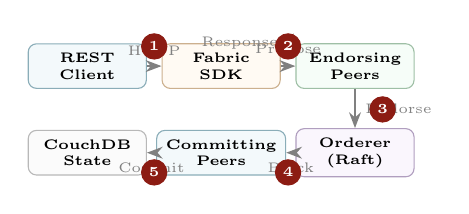
\begin{tikzpicture}[
  step/.style={rectangle, draw=#1!80!black, fill=#1!15, rounded corners=3pt,
               font=\tiny\bfseries, align=center, minimum width=1.5cm, minimum height=0.55cm},
  arr/.style={-{Stealth[length=2mm]}, thick, gray},
  num/.style={circle, draw=asumaroon, fill=asumaroon, text=white, font=\tiny\bfseries,
              inner sep=1pt, minimum size=0.32cm},
]
  \node[step=nodeblue]   (c)   at (0,0)    {REST\\Client};
  \node[step=nodeorange] (sdk) at (1.7,0)  {Fabric\\SDK};
  \node[step=nodegreen]  (ep)  at (3.4,0)  {Endorsing\\Peers};
  \node[step=nodepurple] (ord) at (3.4,-1.1){Orderer\\(Raft)};
  \node[step=nodeblue]   (vp)  at (1.7,-1.1){Committing\\Peers};
  \node[step=nodegray]   (db)  at (0,-1.1) {CouchDB\\State};

  \draw[arr] (c)   -- node[above,font=\tiny]{HTTP} (sdk);
  \draw[arr] (sdk) -- node[above,font=\tiny]{Propose} (ep);
  \draw[arr] (ep)  -- node[right,font=\tiny]{Endorse} (ord);
  \draw[arr] (ord) -- node[below,font=\tiny]{Block} (vp);
  \draw[arr] (vp)  -- node[below,font=\tiny]{Commit} (db);
  \draw[arr, dashed, gray] (ep) to[bend right=20] node[left,font=\tiny]{Response} (sdk);

  % Step numbers
  \node[num] at (0.85, 0.25) {1};
  \node[num] at (2.55, 0.25) {2};
  \node[num] at (3.75,-0.55) {3};
  \node[num] at (2.55,-1.35) {4};
  \node[num] at (0.85,-1.35) {5};
\end{tikzpicture}
\caption{Execute-Order-Validate transaction pipeline.}
\label{fig:txflow}
\end{figure}

\subsection{On-Chain vs.\ Off-Chain Data Design}

Fig.~\ref{fig:onoffchain} visualizes the data partitioning strategy between the ledger and external storage.

\begin{figure}[htbp]
\centering
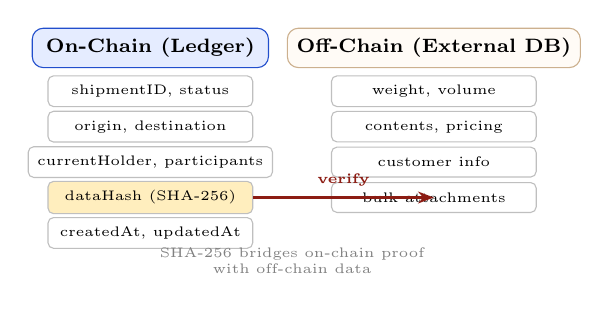
\begin{tikzpicture}[
  store/.style={rectangle, draw=#1!80!black, fill=#1!12, rounded corners=4pt,
                font=\scriptsize\bfseries, minimum width=3cm, minimum height=0.5cm, align=center},
  item/.style={rectangle, draw=gray!50, fill=white, rounded corners=2pt,
               font=\tiny, minimum width=2.6cm, minimum height=0.38cm, align=center},
  arr/.style={-{Stealth[length=2mm]}, thick},
  lbl/.style={font=\tiny\bfseries},
]
  % On-chain block
  \node[store=fabricblue] (on) at (-1.5,0) {On-Chain (Ledger)};
  \node[item] (i1) at (-1.5,-0.55) {shipmentID, status};
  \node[item] (i2) at (-1.5,-1.0)  {origin, destination};
  \node[item] (i3) at (-1.5,-1.45) {currentHolder, participants};
  \node[item, fill=asugold!30] (i4) at (-1.5,-1.9) {dataHash (SHA-256)};
  \node[item] (i5) at (-1.5,-2.35) {createdAt, updatedAt};

  % Off-chain block
  \node[store=nodeorange] (off) at (2.1,0) {Off-Chain (External DB)};
  \node[item] (o1) at (2.1,-0.55) {weight, volume};
  \node[item] (o2) at (2.1,-1.0)  {contents, pricing};
  \node[item] (o3) at (2.1,-1.45) {customer info};
  \node[item] (o4) at (2.1,-1.9)  {bulk attachments};

  % Hash arrow
  \draw[arr, asumaroon, very thick]
    (i4.east) -- node[above, font=\tiny\bfseries, text=asumaroon]{verify} (2.1,-1.9);
  \node[font=\tiny, text=gray, align=center] at (0.3,-2.7)
    {SHA-256 bridges on-chain proof\\with off-chain data};
\end{tikzpicture}
\caption{On-chain vs.\ off-chain data partitioning.}
\label{fig:onoffchain}
\end{figure}

% ════════════════════════════════════════════════════════════════
%  IV. IMPLEMENTATION DETAILS
% ════════════════════════════════════════════════════════════════
\section{Implementation Details}

\subsection{Shipment Lifecycle State Machine}

Fig.~\ref{fig:statemachine} shows the finite state machine governing shipment status transitions.

\begin{figure}[htbp]
\centering
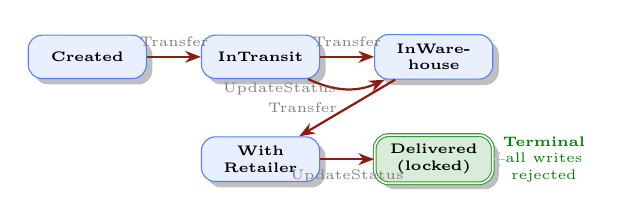
\begin{tikzpicture}[
  state/.style={rectangle, draw=fabricblue!80, fill=fabricblue!10, rounded corners=5pt,
                font=\tiny\bfseries, align=center, minimum width=1.5cm, minimum height=0.55cm,
                drop shadow},
  final/.style={rectangle, draw=darkgreen!80, fill=darkgreen!15, rounded corners=5pt,
                font=\tiny\bfseries, align=center, minimum width=1.5cm, minimum height=0.55cm,
                double, drop shadow},
  arr/.style={-{Stealth[length=2mm]}, thick, asumaroon},
  lbl/.style={font=\tiny, text=gray},
]
  \node[state]  (cr) at (0,0)      {Created};
  \node[state]  (it) at (2.2,0)    {InTransit};
  \node[state]  (iw) at (4.4,0)    {InWare-\\house};
  \node[state]  (wr) at (2.2,-1.3) {With\\Retailer};
  \node[final]  (dl) at (4.4,-1.3) {Delivered\\(locked)};

  \draw[arr] (cr) -- node[above,lbl]{Transfer} (it);
  \draw[arr] (it) -- node[above,lbl]{Transfer} (iw);
  \draw[arr] (iw) -- node[left, lbl]{Transfer} (wr);
  \draw[arr] (wr) -- node[below,lbl]{UpdateStatus} (dl);
  \draw[arr] (it) to[bend right=25] node[left,lbl]{UpdateStatus} (iw);

  % Lock annotation
  \node[font=\tiny, text=darkgreen, align=center] at (5.8,-1.3)
    {\textbf{Terminal}\\all writes\\rejected};
  \draw[->, gray!50, dashed] (5.3,-1.3) -- (dl.east);
\end{tikzpicture}
\caption{Shipment status finite state machine. \textit{Delivered} is a terminal state.}
\label{fig:statemachine}
\end{figure}

\subsection{Smart Contract Functions}

Table~\ref{tab:functions} lists all 10 public chaincode functions.

\begin{table}[htbp]
\centering
\caption{Smart contract functions.}
\label{tab:functions}
\scriptsize
\begin{tabularx}{\columnwidth}{lX}
\toprule
\textbf{Function} & \textbf{Description} \\
\midrule
\texttt{InitLedger} & Seeds a sample shipment for demonstration \\
\texttt{CreateShipment} & Registers a new shipment; caller = initial holder \\
\texttt{GetShipment} & Returns shipment details (participants only) \\
\texttt{UpdateStatus} & Changes status (current holder only) \\
\texttt{TransferCustody} & Transfers to next party (current holder only) \\
\texttt{VerifyShipment} & SHA-256 hash comparison for integrity \\
\texttt{GetHistory} & Returns full event timeline \\
\texttt{AuthorizeParticipant} & Adds party to authorized list \\
\texttt{RevokeParticipant} & Removes party (cannot self-revoke) \\
\texttt{GetAllShipments} & Returns all shipments on ledger \\
\bottomrule
\end{tabularx}
\end{table}

\subsection{RBAC Access Control Model}

Fig.~\ref{fig:rbac} maps each chaincode operation to the caller roles permitted to invoke it.

\begin{figure}[htbp]
\centering
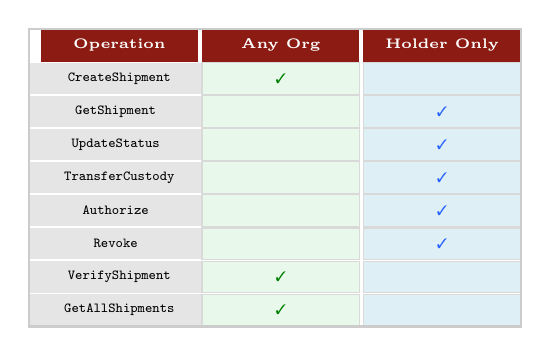
\begin{tikzpicture}[
  hdr/.style={rectangle, fill=asumaroon, text=white, font=\tiny\bfseries,
              minimum width=2cm, minimum height=0.42cm, align=center},
  cell/.style={rectangle, draw=gray!30, fill=#1, font=\tiny,
               minimum width=2cm, minimum height=0.4cm, align=center},
  lhdr/.style={rectangle, fill=gray!20, font=\tiny\bfseries,
               minimum width=2.3cm, minimum height=0.4cm, align=left, inner sep=3pt},
]
  % Header row
  \node[hdr] (h0) at (0,0)    {Operation};
  \node[hdr] (h1) at (2.05,0) {Any Org};
  \node[hdr] (h2) at (4.1,0)  {Holder Only};

  % Rows
  \foreach \op/\any/\holder/\y in {
    CreateShipment/\cmark/ /   -0.42,
    GetShipment   /      /\cmark/-0.84,
    UpdateStatus  /      /\cmark/-1.26,
    TransferCustody/     /\cmark/-1.68,
    Authorize     /      /\cmark/-2.10,
    Revoke        /      /\cmark/-2.52,
    VerifyShipment/\cmark/ /   -2.94,
    GetAllShipments/\cmark/ /  -3.36
  }{
    \node[lhdr] at (0,\y)    {\texttt{\op}};
    \node[cell=nodegreen!40] at (2.05,\y) {\textcolor{darkgreen}{\any}};
    \node[cell=nodeblue!40]  at (4.1,\y)  {\textcolor{fabricblue}{\holder}};
  }
  \draw[thick, gray!40] (-1.15,0.21) rectangle (5.1,-3.57);
\end{tikzpicture}
\caption{RBAC matrix: which caller roles may invoke each operation.}
\label{fig:rbac}
\end{figure}

\subsection{SHA-256 Integrity Verification Flow}

Fig.~\ref{fig:sha256} illustrates how off-chain data authenticity is verified on-chain.

\begin{figure}[htbp]
\centering
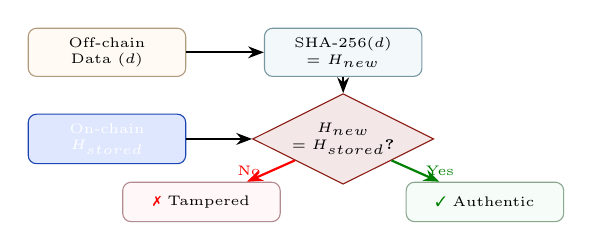
\begin{tikzpicture}[
  box/.style={rectangle, draw=#1!70!black, fill=#1!15, rounded corners=3pt,
              font=\tiny, align=center, minimum width=2cm, minimum height=0.5cm},
  arr/.style={-{Stealth[length=2mm]}, thick},
  decision/.style={diamond, draw=asumaroon, fill=asumaroon!10, font=\tiny\bfseries,
                   align=center, inner sep=1pt, aspect=2},
]
  \node[box=nodeorange] (od) at (0,0)      {Off-chain\\Data ($d$)};
  \node[box=nodeblue]   (hs) at (3,0)      {SHA-256($d$)\\= $H_{new}$};
  \node[box=fabricblue, text=white] (oc) at (0,-1.1) {On-chain\\$H_{stored}$};
  \node[decision] (cmp) at (3,-1.1)        {$H_{new}$\\$=H_{stored}$?};
  \node[box=nodegreen]  (ok)  at (4.8,-1.9){\textcolor{darkgreen}{\cmark} Authentic};
  \node[box=nodered]    (bad) at (1.2,-1.9){\textcolor{red}{\xmark} Tampered};

  \draw[arr] (od) -- (hs);
  \draw[arr] (oc) -- (cmp);
  \draw[arr] (hs) -- (cmp);
  \draw[arr, darkgreen] (cmp) -- node[right,font=\tiny]{Yes} (ok);
  \draw[arr, red]       (cmp) -- node[left, font=\tiny]{No}  (bad);
\end{tikzpicture}
\caption{SHA-256 off-chain data integrity verification flow.}
\label{fig:sha256}
\end{figure}

\subsection{Composite Key Event Storage}

Fig.~\ref{fig:compkey} shows how shipment events are stored using Fabric composite keys for efficient range queries.

\begin{figure}[htbp]
\centering
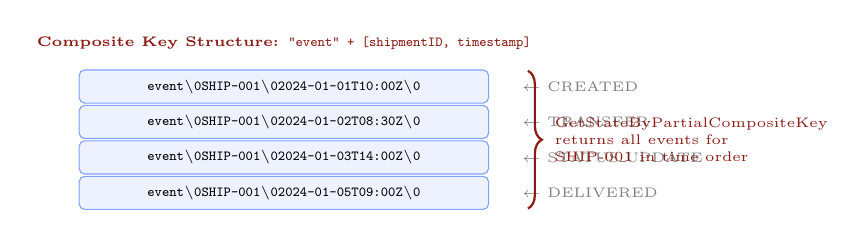
\begin{tikzpicture}[
  key/.style={rectangle, draw=fabricblue!60, fill=fabricblue!8, rounded corners=2pt,
              font=\tiny\ttfamily, align=left, inner sep=3pt,
              minimum width=5.2cm, minimum height=0.42cm},
  lbl/.style={font=\tiny\bfseries, text=asumaroon},
  sub/.style={font=\tiny, text=gray},
]
  \node[lbl] at (0,0) {Composite Key Structure: \texttt{"event" + [shipmentID, timestamp]}};

  \node[key] at (0,-0.55) {event\textbackslash 0SHIP-001\textbackslash 02024-01-01T10:00Z\textbackslash 0};
  \node[sub, right=-0.1cm] at (3.0,-0.55) {$\leftarrow$ CREATED};

  \node[key] at (0,-1.0)  {event\textbackslash 0SHIP-001\textbackslash 02024-01-02T08:30Z\textbackslash 0};
  \node[sub, right=-0.1cm] at (3.0,-1.0)  {$\leftarrow$ TRANSFER};

  \node[key] at (0,-1.45) {event\textbackslash 0SHIP-001\textbackslash 02024-01-03T14:00Z\textbackslash 0};
  \node[sub, right=-0.1cm] at (3.0,-1.45) {$\leftarrow$ STATUS\_UPDATE};

  \node[key] at (0,-1.9)  {event\textbackslash 0SHIP-001\textbackslash 02024-01-05T09:00Z\textbackslash 0};
  \node[sub, right=-0.1cm] at (3.0,-1.9)  {$\leftarrow$ DELIVERED};

  \draw[decorate, decoration={brace,amplitude=5pt}, thick, asumaroon]
    (3.1,-0.35) -- (3.1,-2.1) node[midway, right=6pt, font=\tiny, align=left]
    {GetStateByPartialCompositeKey\\returns all events for\\SHIP-001 in time order};
\end{tikzpicture}
\caption{Composite key layout enabling efficient per-shipment event range queries.}
\label{fig:compkey}
\end{figure}

\subsection{REST API to Chaincode Mapping}

Fig.~\ref{fig:apiflow} shows how HTTP requests map through the Express server to chaincode invocations.

\begin{figure}[htbp]
\centering
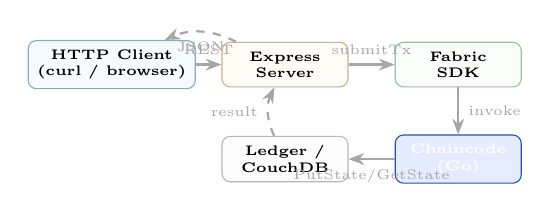
\begin{tikzpicture}[
  layer/.style={rectangle, draw=#1!80!black, fill=#1!12, rounded corners=3pt,
                font=\tiny\bfseries, align=center, minimum width=1.6cm, minimum height=0.5cm},
  ep/.style={rectangle, draw=gray!50, fill=white, font=\tiny, align=left,
             minimum width=2.5cm, minimum height=0.38cm, inner sep=2pt},
  arr/.style={-{Stealth[length=2mm]}, thick, gray!70},
]
  \node[layer=nodeblue]   (cli) at (0,0)   {HTTP Client\\(curl / browser)};
  \node[layer=nodeorange] (exp) at (2.2,0) {Express\\Server};
  \node[layer=nodegreen]  (sdk) at (4.4,0) {Fabric\\SDK};
  \node[layer=fabricblue, text=white] (cc) at (4.4,-1.2) {Chaincode\\(Go)};
  \node[layer=nodegray]   (ld)  at (2.2,-1.2) {Ledger /\\CouchDB};

  \draw[arr] (cli) -- node[above,font=\tiny]{REST} (exp);
  \draw[arr] (exp) -- node[above,font=\tiny]{submitTx} (sdk);
  \draw[arr] (sdk) -- node[right,font=\tiny]{invoke} (cc);
  \draw[arr] (cc)  -- node[below,font=\tiny]{PutState/GetState} (ld);
  \draw[arr, dashed] (ld) to[bend left=25] node[left,font=\tiny]{result} (exp);
  \draw[arr, dashed] (exp) to[bend right=25] node[below,font=\tiny]{JSON} (cli);
\end{tikzpicture}
\caption{REST API to chaincode invocation flow.}
\label{fig:apiflow}
\end{figure}

Table~\ref{tab:api} lists all 10 REST endpoints.

\begin{table}[htbp]
\centering
\caption{REST API endpoints.}
\label{tab:api}
\scriptsize
\begin{tabularx}{\columnwidth}{llX}
\toprule
\textbf{Method} & \textbf{Endpoint} & \textbf{Function} \\
\midrule
POST   & /api/shipments                    & CreateShipment \\
GET    & /api/shipments                    & GetAllShipments \\
GET    & /api/shipments/:id                & GetShipment \\
PUT    & /api/shipments/:id/status         & UpdateStatus \\
PUT    & /api/shipments/:id/transfer       & TransferCustody \\
GET    & /api/shipments/:id/verify         & VerifyShipment \\
GET    & /api/shipments/:id/history        & GetHistory \\
POST   & /api/shipments/:id/participants   & Authorize \\
DELETE & /api/shipments/:id/participants/:p & Revoke \\
GET    & /api/health                       & Health check \\
\bottomrule
\end{tabularx}
\end{table}

% ════════════════════════════════════════════════════════════════
%  V. RESULTS
% ════════════════════════════════════════════════════════════════
\section{Results}

\subsection{Unit Test Results}

We implemented 15 unit tests using Go's \texttt{testing} package with Fabric's \texttt{shimtest.MockStub}. A key challenge was that MockStub does not natively support client identity extraction. We resolved this by injecting mock creator identities using \texttt{mspproto.SerializedIdentity} with self-signed X.509 certificates via Go's \texttt{crypto/x509} library. All 15 tests pass in 0.437 seconds (Table~\ref{tab:tests}).

\begin{table}[htbp]
\centering
\caption{Unit test results---15/15 passed (0.437s).}
\label{tab:tests}
\scriptsize
\begin{tabularx}{\columnwidth}{clX}
\toprule
\# & \textbf{P/F} & \textbf{Test Case} \\
\midrule
1  & \textcolor{darkgreen}{\cmark} & InitLedger---sample data seeded \\
2  & \textcolor{darkgreen}{\cmark} & CreateShipment---new shipment created \\
3  & \textcolor{darkgreen}{\cmark} & CreateShipmentDuplicate---rejected \\
4  & \textcolor{darkgreen}{\cmark} & UpdateShipmentStatus---valid update \\
5  & \textcolor{darkgreen}{\cmark} & UpdateStatusInvalid---bad status rejected \\
6  & \textcolor{darkgreen}{\cmark} & TransferCustody---successful transfer \\
7  & \textcolor{darkgreen}{\cmark} & TransferUnauthorized---blocked \\
8  & \textcolor{darkgreen}{\cmark} & VerifyShipmentValid---data authentic \\
9  & \textcolor{darkgreen}{\cmark} & VerifyShipmentInvalid---tampering detected \\
10 & \textcolor{darkgreen}{\cmark} & AuthorizeParticipant---added \\
11 & \textcolor{darkgreen}{\cmark} & RevokeParticipant---removed \\
12 & \textcolor{darkgreen}{\cmark} & FullLifecycle---end-to-end flow \\
13 & \textcolor{darkgreen}{\cmark} & DeliveredLocked---writes rejected \\
14 & \textcolor{darkgreen}{\cmark} & GetAllShipments---retrieval works \\
15 & \textcolor{darkgreen}{\cmark} & ComputeHash---SHA-256 correct \\
\bottomrule
\end{tabularx}
\end{table}

Fig.~\ref{fig:testcoverage} visualizes test coverage by functional area.

\begin{figure}[htbp]
\centering
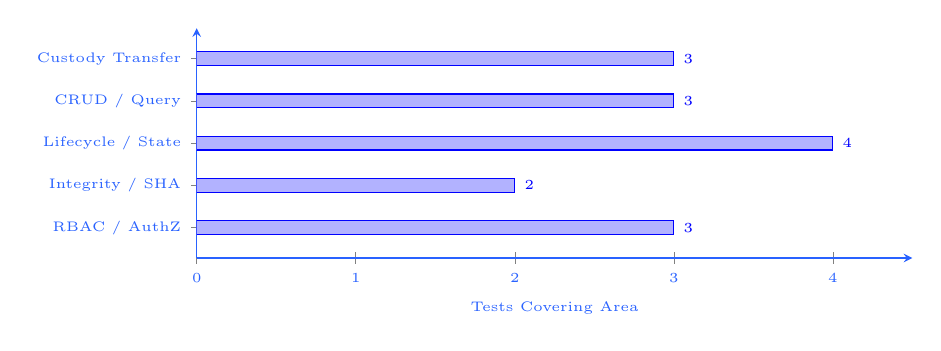
\begin{tikzpicture}
\begin{axis}[
    xbar,
    width=\columnwidth*0.88,
    height=4.5cm,
    bar width=5pt,
    xmin=0, xmax=4.5,
    xlabel={\tiny Tests Covering Area},
    xtick={0,1,2,3,4},
    ytick=data,
    yticklabels={
      {RBAC / AuthZ},
      {Integrity / SHA},
      {Lifecycle / State},
      {CRUD / Query},
      {Custody Transfer}
    },
    yticklabel style={font=\tiny},
    xlabel style={font=\tiny},
    nodes near coords,
    nodes near coords style={font=\tiny},
    every axis/.append style={font=\tiny},
    axis lines=left,
    enlarge y limits=0.18,
    bar shift=0pt,
    color=fabricblue,
    fill=fabricblue!40,
]
\addplot coordinates {(3,0) (2,1) (4,2) (3,3) (3,4)};
\end{axis}
\end{tikzpicture}
\caption{Unit test coverage by functional area (15 tests total).}
\label{fig:testcoverage}
\end{figure}

\subsection{End-to-End Lifecycle Validation}

The \texttt{TestFullLifecycle} test validates the complete business flow across 4 organizational identities: (1)~initialize ledger, (2)~create shipment, (3)~transfer Manufacturer$\to$Transporter, (4)~transfer Transporter$\to$Warehouse, (5)~update status to InWarehouse, (6)~transfer Warehouse$\to$Retailer, (7)~mark Delivered, (8)~verify post-delivery updates are rejected, and (9)~verify post-delivery transfers are rejected. This single test exercises 7 of the 10 chaincode functions.

Fig.~\ref{fig:custodyseq} illustrates the custody transfer sequence across organizations.

\begin{figure}[htbp]
\centering
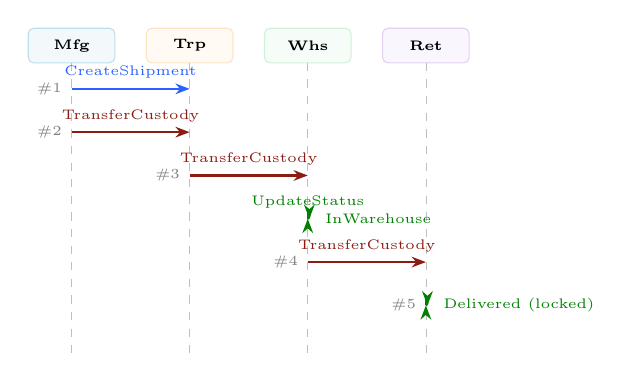
\begin{tikzpicture}[
  actor/.style={rectangle, draw=#1!80, fill=#1!15, rounded corners=2pt,
                font=\tiny\bfseries, align=center, minimum width=1.1cm, minimum height=0.44cm},
  msg/.style={-{Stealth[length=1.8mm]}, thick, #1},
  lifeline/.style={dashed, gray!50, very thin},
  evt/.style={font=\tiny, text=#1},
]
  % Actors
  \node[actor=nodeblue]   (mfg) at (0,0)   {Mfg};
  \node[actor=nodeorange] (trp) at (1.5,0) {Trp};
  \node[actor=nodegreen]  (whs) at (3.0,0) {Whs};
  \node[actor=nodepurple] (ret) at (4.5,0) {Ret};

  % Lifelines
  \foreach \x in {0,1.5,3.0,4.5}
    \draw[lifeline] (\x,-0.22) -- (\x,-4.0);

  % Messages
  \draw[msg=fabricblue] (0,-0.55) -- node[above,evt=fabricblue]{CreateShipment} (1.5,-0.55);
  \node[evt=gray, left] at (0,-0.55) {\tiny \#1};

  \draw[msg=asumaroon] (0,-1.1) -- node[above,evt=asumaroon]{TransferCustody} (1.5,-1.1);
  \node[evt=gray, left] at (0,-1.1) {\tiny \#2};

  \draw[msg=asumaroon] (1.5,-1.65) -- node[above,evt=asumaroon]{TransferCustody} (3.0,-1.65);
  \node[evt=gray, left] at (1.5,-1.65) {\tiny \#3};

  \draw[msg=darkgreen] (3.0,-2.2) -- node[above,evt=darkgreen]{UpdateStatus} (3.0,-2.2);
  \draw[-{Stealth[length=1.8mm]}, thick, darkgreen] (3.0,-2.2) arc(180:0:0.01);
  \node[evt=darkgreen, right=0.1cm] at (3.0,-2.2) {\tiny InWarehouse};

  \draw[msg=asumaroon] (3.0,-2.75) -- node[above,evt=asumaroon]{TransferCustody} (4.5,-2.75);
  \node[evt=gray, left] at (3.0,-2.75) {\tiny \#4};

  \draw[msg=darkgreen] (4.5,-3.3) -- (4.5,-3.3);
  \draw[-{Stealth[length=1.8mm]}, thick, darkgreen] (4.5,-3.3) arc(180:0:0.01);
  \node[evt=darkgreen, right=0.1cm] at (4.5,-3.3) {\tiny Delivered (locked)};
  \node[evt=gray, left] at (4.5,-3.3) {\tiny \#5};
\end{tikzpicture}
\caption{Custody transfer sequence across four organizations.}
\label{fig:custodyseq}
\end{figure}

% ════════════════════════════════════════════════════════════════
%  VI. ANALYSIS
% ════════════════════════════════════════════════════════════════
\section{Analysis}

\subsection{Scalability}

Table~\ref{tab:scalability} summarizes scalability characteristics. Fig.~\ref{fig:scalability} plots projected ledger growth.

\begin{table}[htbp]
\centering
\caption{Scalability characteristics.}
\label{tab:scalability}
\scriptsize
\begin{tabularx}{\columnwidth}{lX}
\toprule
\textbf{Factor} & \textbf{Assessment} \\
\midrule
Tx payload  & Small ($<$1\,KB): metadata + hash only; avoids ledger bloat. \\
Throughput  & 2,000--3,500 TPS (Fabric 2.5, 2 orgs, Raft) \cite{fabricdocs}. \\
State DB    & CouchDB indexing; \texttt{GetAllShipments} degrades at $>$10K records without pagination. \\
Event growth & Linear: $n$ lifecycle events $\Rightarrow$ $n$ ledger entries per shipment. \\
Horizontal  & Add peers per org; 3--5 Raft orderers for CFT. \\
\bottomrule
\end{tabularx}
\end{table}

\begin{figure}[htbp]
\centering
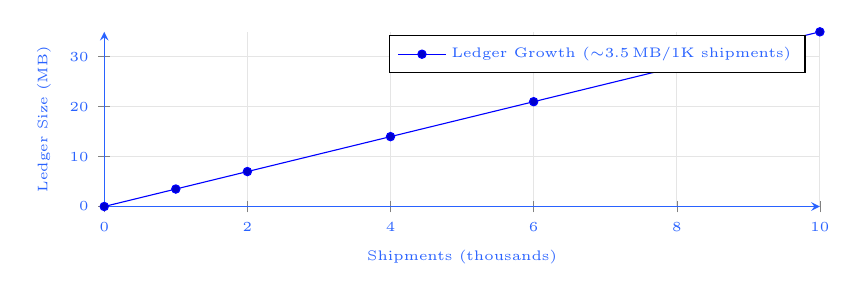
\begin{tikzpicture}
\begin{axis}[
    width=\columnwidth*0.88,
    height=3.8cm,
    xlabel={\tiny Shipments (thousands)},
    ylabel={\tiny Ledger Size (MB)},
    xlabel style={font=\tiny},
    ylabel style={font=\tiny},
    xtick={0,2,4,6,8,10},
    ytick={0,10,20,30,40},
    xticklabel style={font=\tiny},
    yticklabel style={font=\tiny},
    axis lines=left,
    grid=major,
    grid style={gray!20},
    mark=*,
    mark size=1.5pt,
    color=fabricblue,
]
\addplot coordinates {(0,0)(1,3.5)(2,7)(4,14)(6,21)(8,28)(10,35)};
\addlegendentry{\tiny Ledger Growth ($\sim$3.5\,MB/1K shipments)}
\end{axis}
\end{tikzpicture}
\caption{Projected ledger growth at $\sim$10 events/shipment, 300 bytes/event.}
\label{fig:scalability}
\end{figure}

\subsection{Transaction Cost Analysis}

Table~\ref{tab:costs} compares cost structures between Ethereum and our Fabric deployment.

\begin{table}[htbp]
\centering
\caption{Transaction cost comparison.}
\label{tab:costs}
\scriptsize
\begin{tabularx}{\columnwidth}{lXX}
\toprule
\textbf{Cost Factor} & \textbf{Ethereum (Public)} & \textbf{Fabric (Ours)} \\
\midrule
Per-tx fee    & \$0.50--\$50+ (gas)         & \$0 (no gas) \\
Infrastructure & None (public network)       & Docker hosts per org \\
Monthly est.  & \$15K--\$150K at 10K tx/day & \$500--\$2,000 (cloud VMs) \\
Identity mgmt.& MetaMask wallets             & Fabric CA (X.509 PKI) \\
Finality time & $\sim$12\,s (PoS)           & $\sim$0.5--2\,s (Raft) \\
\bottomrule
\end{tabularx}
\end{table}

\subsection{Blockchain vs.\ Traditional Database}

Fig.~\ref{fig:radar} provides a visual spider-chart comparison across six dimensions.

\begin{figure}[htbp]
\centering
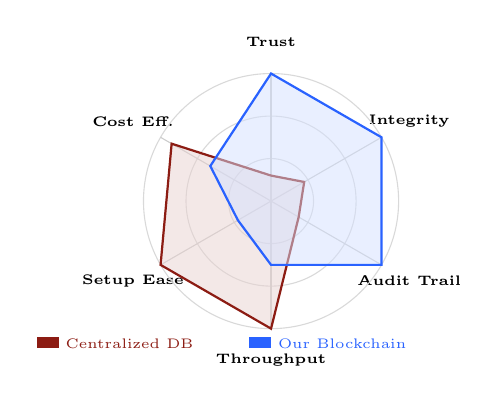
\begin{tikzpicture}[scale=0.9]
  % Axes: Trust, Integrity, Audit, Throughput(inv), Setup-ease(inv), Cost-eff
  \def\N{6}
  \def\R{1.8}

  % Axis labels
  \foreach \lbl/\ang in {
    Trust/90,
    Integrity/30,
    {Audit Trail}/330,
    {Throughput}/270,
    {Setup Ease}/210,
    {Cost Eff.}/150
  }{
    \node[font=\tiny\bfseries] at (\ang:\R*1.25) {\lbl};
  }

  % Grid circles
  \foreach \r in {0.6,1.2,1.8}{
    \draw[gray!30] (0,0) circle (\r);
  }

  % Axes
  \foreach \ang in {90,30,330,270,210,150}
    \draw[gray!40] (0,0) -- (\ang:\R);

  % Centralized DB values (normalized 0-1 * R):
  % Trust=0.2, Integrity=0.3, Audit=0.25, Throughput=1.0, SetupEase=1.0, CostEff=0.9
  \draw[thick, asumaroon, fill=asumaroon!20, fill opacity=0.5]
    (90:0.2*\R) -- (30:0.3*\R) -- (330:0.25*\R) --
    (270:1.0*\R) -- (210:1.0*\R) -- (150:0.9*\R) -- cycle;

  % Our Blockchain values:
  % Trust=1.0, Integrity=1.0, Audit=1.0, Throughput=0.5, SetupEase=0.3, CostEff=0.55
  \draw[thick, fabricblue, fill=fabricblue!20, fill opacity=0.5]
    (90:1.0*\R) -- (30:1.0*\R) -- (330:1.0*\R) --
    (270:0.5*\R) -- (210:0.3*\R) -- (150:0.55*\R) -- cycle;

  % Legend
  \node[font=\tiny, asumaroon] at (-2.2,-2.0) {\rule{8pt}{4pt} Centralized DB};
  \node[font=\tiny, fabricblue] at (0.8,-2.0)  {\rule{8pt}{4pt} Our Blockchain};
\end{tikzpicture}
\caption{Radar comparison: blockchain vs.\ centralized database across six criteria.}
\label{fig:radar}
\end{figure}

\subsection{Privacy and Regulatory Considerations}

\begin{table}[htbp]
\centering
\caption{Privacy and regulatory analysis.}
\label{tab:privacy}
\scriptsize
\begin{tabularx}{\columnwidth}{lX}
\toprule
\textbf{Concern} & \textbf{How Addressed} \\
\midrule
Data visibility   & Fabric channels + RBAC restrict per-shipment access. \\
GDPR Art.~17      & Personal data off-chain; only pseudonymous hashes on-chain. \\
Data minimization & Sensitive details (contents, pricing) remain off-chain. \\
Cross-border      & Each org hosts its own peer within its jurisdiction. \\
Audit compliance  & Signed, timestamped history satisfies SOX, FDA 21 CFR Part~11. \\
\bottomrule
\end{tabularx}
\end{table}

% ════════════════════════════════════════════════════════════════
%  VII. INNOVATION & IMPACT
% ════════════════════════════════════════════════════════════════
\section{Innovation and Impact}

\subsection{Design Innovations}

\begin{itemize}[nosep, leftmargin=*]
    \item \textbf{Dynamic participant authorization:} Current holder can authorize/revoke parties mid-transit (e.g., adding an insurance auditor).
    \item \textbf{SHA-256 off-chain bridge:} Mathematical verification of off-chain data without trusting the data provider.
    \item \textbf{Delivered-state immutability:} Terminal state permanently rejects all writes at chaincode level.
    \item \textbf{Composite-key event history:} Efficient per-shipment range queries without full ledger scans.
\end{itemize}

\subsection{Practical Impact}

\textbf{Target industries:} Pharmaceuticals (FDA track-and-trace), food safety, luxury goods (anti-counterfeiting), and general logistics. A production deployment requires 5+ peer organizations, a 3--5 node Raft cluster, ERP/WMS middleware, and a web dashboard.

% ════════════════════════════════════════════════════════════════
%  VIII. CHALLENGES AND LIMITATIONS
% ════════════════════════════════════════════════════════════════
\section{Challenges and Limitations}

\subsection{Technical Challenges}

\begin{enumerate}[nosep, leftmargin=*]
    \item \textbf{Mock Identity in Tests:} Solved with \texttt{mspproto.SerializedIdentity} and self-signed X.509 certs via \texttt{crypto/x509}.
    \item \textbf{Go Module Dependencies:} Fabric's transitive dependency tree requires careful \texttt{go.mod} management.
    \item \textbf{Network Configuration:} Multi-org setup demands consistent naming across Docker Compose, crypto config, and channel config.
\end{enumerate}

\subsection{Current Limitations}

Two organizations only (demo); no GUI; single orderer; no IPFS; no pagination in \texttt{GetAllShipments()}.

% ════════════════════════════════════════════════════════════════
%  IX. FUTURE WORK
% ════════════════════════════════════════════════════════════════
\section{Future Work}

\begin{enumerate}[nosep, leftmargin=*]
    \item \textbf{Private Data Collections:} Bilateral sensitive data sharing without channel-wide exposure.
    \item \textbf{IPFS Integration:} Content-addressed off-chain storage.
    \item \textbf{Paginated Queries:} CouchDB bookmark-based pagination for high-volume deployments.
    \item \textbf{IoT Integration:} GPS/temperature sensors for automated status updates.
    \item \textbf{Frontend Dashboard:} React/Next.js web application for real-time visualization.
    \item \textbf{Performance Benchmarking:} Hyperledger Caliper for TPS, latency, and resource profiling.
    \item \textbf{Multi-orderer Cluster:} 3--5 Raft orderers for production fault tolerance.
\end{enumerate}

% ════════════════════════════════════════════════════════════════
%  X. CONCLUSION
% ════════════════════════════════════════════════════════════════
\section{Conclusion}

This paper presented a blockchain-based shipment tracking system on Hyperledger Fabric 2.5 addressing the fundamental trust deficit in multi-organization supply chains. Our Go chaincode (647 lines, 10 functions) enforces RBAC via MSP identities, maintains data integrity through SHA-256 off-chain hashing, and provides a complete, immutable event history using composite keys. All 15 unit tests pass in 0.437s, confirming correctness across access control, custody transfer, data verification, and post-delivery immutability. While the blockchain approach trades raw throughput (2,000--3,500 vs.\ 10,000+ TPS) for trustlessness and cryptographic auditability, the trade-off is fully justified for multi-organization supply chains where disputes and tampering are significant concerns.

% ════════════════════════════════════════════════════════════════
%  XI. CONTRIBUTIONS
% ════════════════════════════════════════════════════════════════
\section{Team Contributions}

\begin{table}[htbp]
\centering
\caption{Individual team member contributions.}
\scriptsize
\begin{tabularx}{\columnwidth}{lX}
\toprule
\textbf{Member} & \textbf{Contributions} \\
\midrule
D. Agnello & Architecture, repo setup, smart contract design \& implementation \\
R. Abrol   & Network config, Docker Compose, channel \& crypto config \\
V. Patel   & Client app (Node.js REST API), SDK integration \\
S. Nanda   & Unit testing, mock identity, report, analysis \\
A. Bhure   & Research, literature review, documentation, presentation \\
\bottomrule
\end{tabularx}
\end{table}

% ════════════════════════════════════════════════════════════════
%  REFERENCES
% ════════════════════════════════════════════════════════════════
\balance
\begin{thebibliography}{7}

\bibitem{shakhbulatov2020}
D. Shakhbulatov, J. Medina, Z. Dong and R. Rojas-Cessa, ``How Blockchain Enhances Supply Chain Management: A Survey,'' \textit{IEEE Open Journal of the Computer Society}, vol.~1, pp.~230--249, 2020.

\bibitem{oguz2024}
S. O\u{g}uz, G. Alkan, B. Yilmaz and C. Kocaba\c{s}, ``The Use of Blockchain Technology in Logistics and Supply Chain Management (SCM): A Systematic Review,'' \textit{IEEE Access}, vol.~12, pp.~166211--166224, 2024.

\bibitem{gonczol2020}
P. Gonczol, P. Katsikouli, L. Herskind and N. Dragoni, ``Blockchain Implementations and Use Cases for Supply Chains --- A Survey,'' \textit{IEEE Access}, vol.~8, pp.~11856--11871, 2020.

\bibitem{wang2019}
S. Wang, D. Li, Y. Zhang and J. Chen, ``Smart Contract-Based Product Traceability System in the Supply Chain Scenario,'' \textit{IEEE Access}, vol.~7, pp.~115122--115133, 2019.

\bibitem{fabricdocs}
Hyperledger Fabric Documentation, \url{https://hyperledger-fabric.readthedocs.io/}, accessed April 2026.

\bibitem{fabricapi}
Hyperledger Fabric Contract API for Go, \url{https://pkg.go.dev/github.com/hyperledger/fabric-contract-api-go}.

\bibitem{docker}
Docker Documentation, \url{https://docs.docker.com/}.

\end{thebibliography}

\end{document}
